\documentclass{article}
\usepackage[utf8]{inputenc}
\usepackage[T1]{fontenc}
\usepackage{xcolor}
\usepackage{amsmath}
\usepackage{amssymb}
\usepackage{pgfplots}
\usepackage{tikz}
\usepackage{tcolorbox}
\pgfplotsset{compat=1.18}
\usepgfplotslibrary{fillbetween}
\usetikzlibrary{shapes.misc, positioning, shapes, shadows, patterns}

\begin{document}

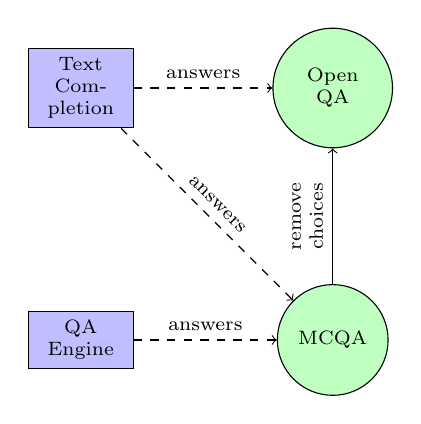
\begin{tikzpicture}[node distance=3.2cm,text width=1.1cm, font=\scriptsize, align=center]
    \node[draw, rectangle, fill=blue!25] (tc) {Text Completion};
    \node[draw, rectangle, fill=blue!25] (qa) [below of=tc] {QA Engine};
    \node[draw, circle, fill=green!25] (op) [right of=tc] {Open QA};
    \node[draw, circle, fill=green!25] (mc) [right of=qa] {MCQA};

    \draw[->, dashed] (tc) -- node[pos=0.5, above]{answers} (op);
    \draw[->, dashed] (tc) -- node[pos=0.5, sloped, above]{answers} (mc);
    \draw[->, dashed] (qa) -- node[pos=0.5, above]{answers} (mc);
    \draw[->] (mc) -- node[pos=0.5, sloped, above]{remove choices} (op);
  \end{tikzpicture}

\end{document}